\newpage

\hypertarget{identituxe4t}{%
\chapter{Identität}\label{identituxe4t}}

Im Rahmen der Vorlesung ``Simulation and Reinforcement Learning'' sollen
drei Fahrstühle eines Bürogebäudes simuliert und anschließend ihre
Funktion mittels Reinforcement Learning optimiert werden.

\begin{figure}
\centering
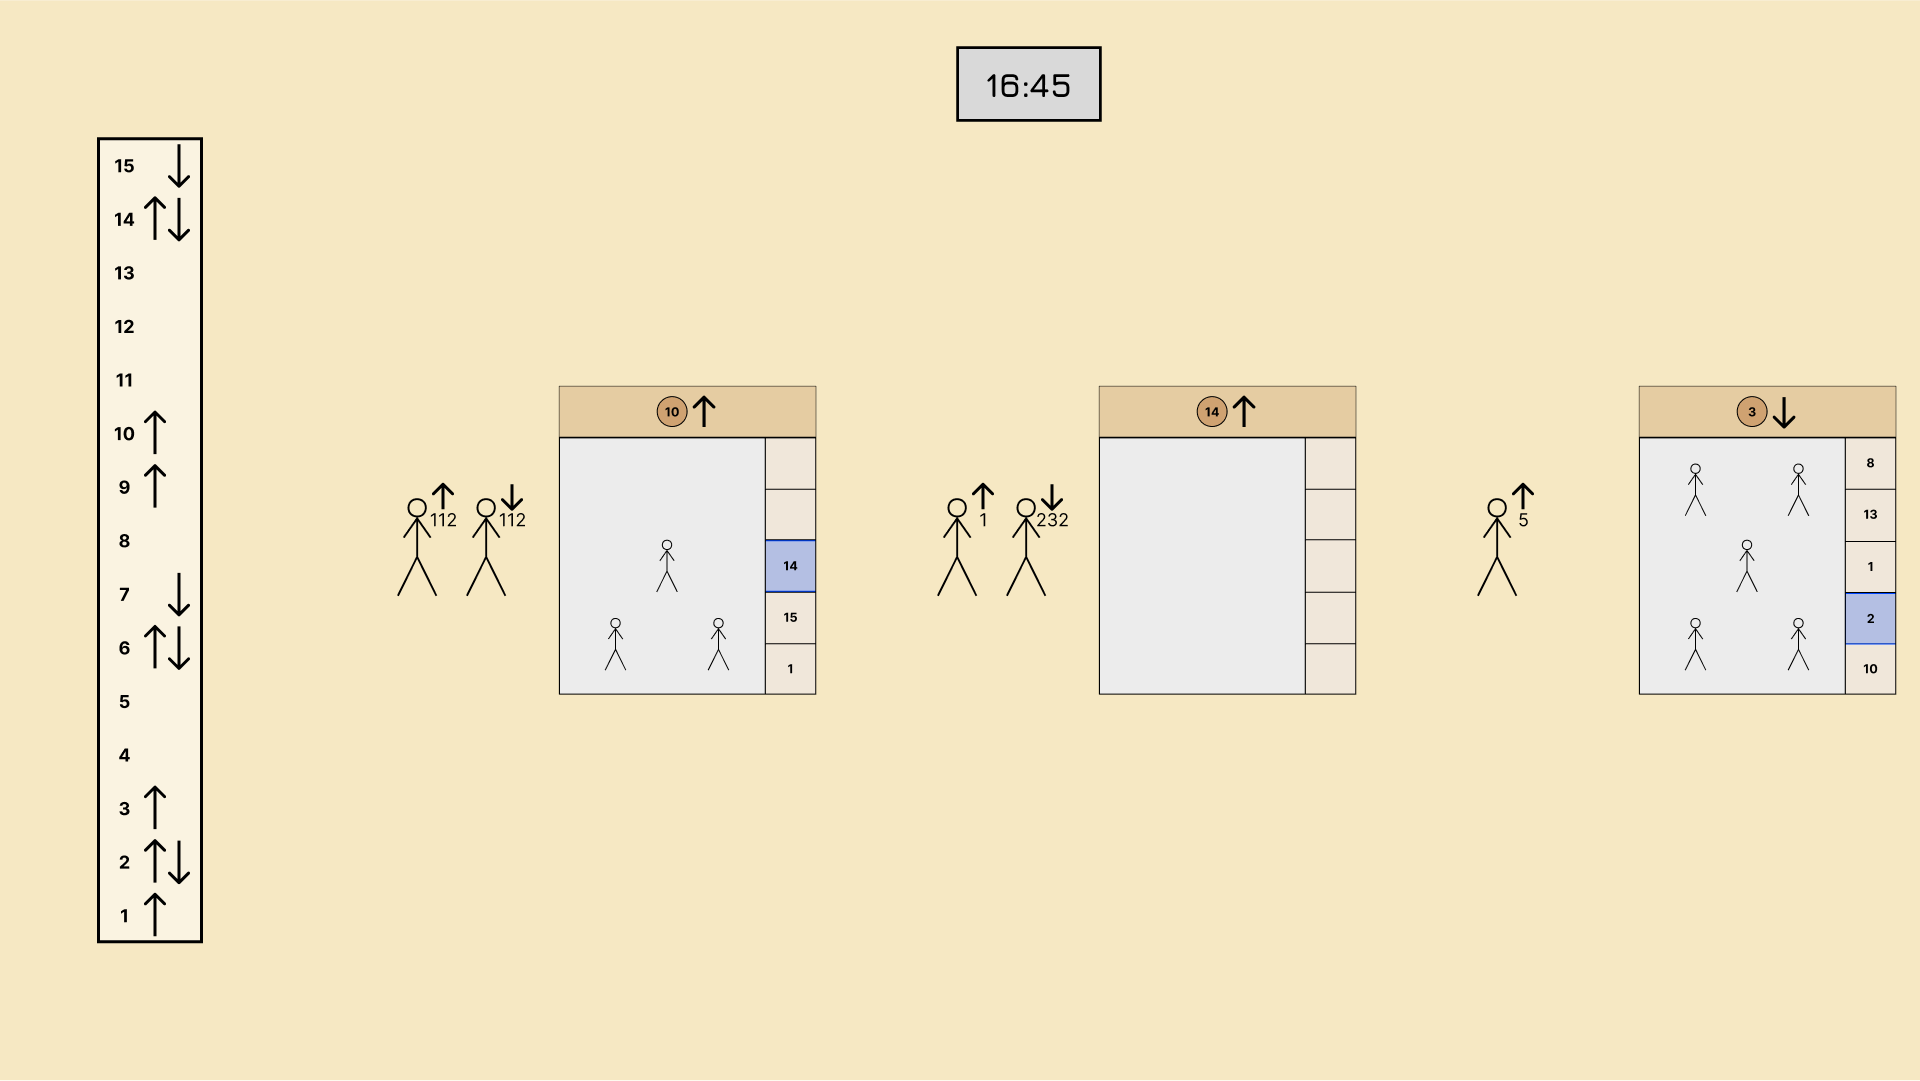
\includegraphics{../images/Fahrstuhl.png}
\caption{UI der späteren Fahrstuhl-Simulation}
\end{figure}

Hierfür wird die Simulation auf einen groben Detailgrad
heruntergebrochen. Die Grenzen der Simulation werden in den
nachfolgenden Kapiteln genauer beleuchtet.

\hypertarget{eigenschaften}{%
\chapter{Eigenschaften}\label{eigenschaften}}

\hypertarget{innere-struktur-des-fahrstuhls}{%
\section{Innere Struktur des
Fahrstuhls}\label{innere-struktur-des-fahrstuhls}}

Der Fahrstuhl ist in 3 Elementen aufgeteilt.

\begin{itemize}
\tightlist
\item
  Stockwerksposition und Fahrtrichtung
\item
  Personenanzahl für nach oben und unten des aktuellen Stockwerks
\item
  Innenraum
\end{itemize}

Der Innenraum zeigt, wie viele Personen sich in ihm befinden und wo
welche Knöpfe in welcher Reihenfolge gedrückt wurden. Des Weiteren wird
sein Fahrziel hervorgehoben angezeigt.

Es gibt drei Zustände je Fahrstuhl:

\begin{itemize}
\tightlist
\item
  Warten
\item
  Hoch
\item
  Runter
\end{itemize}

Warten fasst zwei Zustände zusammen. Das Warten, bis ein Rufknopf
gedrückt wurde und bis der Ein- und Aussteigevorgang abgeschlossen ist.

\hypertarget{uxe4uuxdfere-parameter.}{%
\section{Äußere Parameter.}\label{uxe4uuxdfere-parameter.}}

Die äußeren Parameter, die sich auf das Modell auswirken, sind die zu
befördernden Personen. Die Fahrstühle kennen lediglich die Anzahl der
Personen in ihrem Inneren und in welchem Stockwerk eine unbekannte
Anzahl an Personen nach oben und / oder nach unten möchten.

\hypertarget{ein--und-ausgabeparameter}{%
\section{Ein- und Ausgabeparameter}\label{ein--und-ausgabeparameter}}

Um das Modell möglichst flexibel zu gestalten, wird eine Bandbreite von
Ein- und Ausgabeparametern unterstützt. Diese können wiederum in
Fahrstuhl, Personen und Haus unterteilt werden.

\hypertarget{eingabeparametern}{%
\subsection{Eingabeparametern:}\label{eingabeparametern}}

Zu den Eingabeparametern der Fahrstühle gehören:

\begin{itemize}
\tightlist
\item
  Kapazität der Fahrstühle
\item
  Geschwindigkeit der Etagenwechsel (in Takten)
\item
  Dauer des Ein- und Aussteigevorgangs (in Takten)
\end{itemize}

Zu den Eingabeparametern des Hauses gehören:

\begin{itemize}
\tightlist
\item
  Anzahl an Etagen
\item
  Liste von Etagen und Zeiten von Spitzenaufkommen (Bspw. Mittagspause).
\end{itemize}

Personen steuern im Gegensatz nur das maximale Tagesaufkommen zu den
Eingaben bei.

\hypertarget{ausgabeparametern}{%
\subsection{Ausgabeparametern:}\label{ausgabeparametern}}

Die Ausgabeparameter beschränken sich außerhalb des Logs lediglich auf
die Aussagen, ob alle Personen bis zum Ende des Tages das Gebäude
verlassen haben und welche durchschnittliche Wartezeit vorliegt.

\hypertarget{verhalten}{%
\chapter{Verhalten}\label{verhalten}}

\hypertarget{vorbedingungen}{%
\section{Vorbedingungen}\label{vorbedingungen}}

\hypertarget{interne-prozesse}{%
\section{Interne Prozesse}\label{interne-prozesse}}

\hypertarget{fehlermuxf6glichkeit}{%
\section{Fehlermöglichkeit}\label{fehlermuxf6glichkeit}}

\hypertarget{nachbedingung}{%
\section{Nachbedingung}\label{nachbedingung}}

\hypertarget{verifikation-und-validierung}{%
\chapter{Verifikation und
Validierung}\label{verifikation-und-validierung}}

\hypertarget{verifikation}{%
\section{Verifikation}\label{verifikation}}

\hypertarget{validierung}{%
\section{Validierung}\label{validierung}}
